\section{Spin and current couplings}\label{sec:10.4}

Dark matter with an anapole moment couples to electrons partly through $\mathcal{O}_8 = \vect{S}_\chi\cdot\vect{v}^\perp$, the dark-matter spin times the relative velocity of the two particles (\cref{sec:8.1}). For an electron at rest the relative velocity equals the velocity of the dark matter, typically $10^{-3}$, and the rate is the density rate of \cref{sec:10.2} times $|\bar{\vect{v}}_{\mathrm{T}}|^2/4$, with $\bar{\vect{v}}_{\mathrm{T}}$ the part of the dark matter's mean velocity across $\vect{q}$. The valence electrons of silicon, however, are not at rest. Taken as a free gas at their density they move at $v_{\mathrm{F}} = 7.0\times10^{-3}$, nine times the dispersion $v_0$ of the halo, and the velocity in $\mathcal{O}_8$ is the difference between the dark-matter velocity and the electron velocity. The electron's own motion couples through the electron current, a separate row of the response matrix, which the medium screens differently from the density. Every coupling beyond the density needs new responses of the crystal, each screened in its own way, and an interference term between rows; the interference term has not been computed.

\subsection{The minimal response table}\label{sec:10.4-table}

The rows of \cref{eq:8.1-rows} for the electrons are the density $n_e$, the spin density $\vect{s}_e$, the current $\vect{j}_e$, the spin current $\mathcal{J}^{\alpha\beta}_e$ and the kinetic-energy density $\mathcal{T}_e$, three of them vectors and one a tensor. Counted by components they are 17 operators, and the response matrix has 289 elements at every $(\vect{q},\omega)$. Three constraints reduce them to a few functions: charge conservation, spin-rotation symmetry and the combined symmetry of inversion and time reversal. \Cref{app:D.30} derives each step.

Charge conservation comes first. For a Hamiltonian with local potentials the current along $\vect{q}$, $j_{\mathrm{L}} = \hat{\vect{q}}\cdot\vect{j}_e$, has the matrix elements of $(\omega/q)\,n_e$ between eigenstates (\cref{eq:4.3-continuity}), and every element of the response matrix that contains $j_{\mathrm{L}}$ is a multiple of one that does not (\cref{eq:D.30-continuity}). On the dark-matter side the same holds for the velocity, $\hat{\vect{q}}\cdot\bar{\vect{v}}_\chi = (\omega + \Delta_\chi)/q$. For elastic dark matter the two longitudinal parts cancel (\cref{eq:8.1-transverse}), and only the transverse current survives, $j_{\mathrm{T}i} = \hat{\vect{e}}_i\cdot\vect{j}_e$ along two unit vectors $\hat{\vect{e}}_{1,2}$ perpendicular to $\vect{q}$. If the electron spin is conserved, the spin current obeys its own continuity equation, and only its transverse velocity components $\mathcal{J}^{\mathrm{T}i,\beta}_e = \hat e^\alpha_i\mathcal{J}^{\alpha\beta}_e$ survive.

Without spin--orbit coupling and without magnetic order the Hamiltonian is unchanged by a rotation of all spins, and the ground state of silicon is a spin singlet. The density, the current and the kinetic-energy density do not act on spin and make singlet pairs; the spin density and the spin current make triplets. Singlet and triplet pairs never interfere, and the response matrix splits into a singlet block on $\{n_e, j_{\mathrm{T}1}, j_{\mathrm{T}2}, \mathcal{T}_e\}$ and a triplet block on $\{s^z_e, \mathcal{J}^{\mathrm{T}1,z}_e, \mathcal{J}^{\mathrm{T}2,z}_e\}$, the same for every spin component. For independent electrons the triplet block is a quarter of the singlet one (\cref{eq:D.30-quarter}): the spin vertex $\sigma^z/2$ has $(\pm\frac12)^2 = \frac14$ where the density vertex has 1, and the spatial sums are the same. The unscreened crystal form factor of \cref{sec:10.1} therefore also gives the spin-dependent rate of $\mathcal{O}_4$ at the independent-particle level, up to the spin traces of the two particles. Beyond independent particles the factor $\frac14$ fails, as the next subsection shows.

Silicon and germanium are also symmetric under inversion combined with time reversal, which makes every element of both blocks real. The singlet block on $\{n_e, j_{\mathrm{T}1}, j_{\mathrm{T}2}\}$ is then a real symmetric $3\times3$ matrix: six real functions of $(\vect{q},\omega)$, namely $S_{nn}$, two density--current elements and three current--current elements. A complete table holds them twice, screened and for independent particles, and the independent-particle set fixes the triplet block at that level. The table then holds twelve functions. Operator $\mathcal{O}_2$ alone needs more: its velocity squared brings in $\mathcal{T}_e$, with four further elements in each version. For $\vect{q}$ along a two-, three- or fourfold axis of the cubic crystal, a rotation about $\hat{\vect{q}}$ leaves the density unchanged and turns the transverse current, so the density--current elements vanish.

\Cref{tab:10-minimal} sorts the operators of \cref{tab:8-operators} by block.

\begin{table}[tbp]
  \caption{The minimal response table: the rows of the electronic response matrix that each non-relativistic operator of \cref{tab:8-operators} needs, and their screening. The longitudinal current and spin current have been eliminated by continuity (elastic scattering, local potentials, electron spin conserved). Screening is for a cubic crystal without spin--orbit coupling or magnetic order. Singlet rows make spin-singlet electron--hole pairs and triplet rows spin-triplet pairs; the two blocks do not interfere. Notation: $j_{\mathrm{T}}$, current across $\vect{q}$; $\mathcal{J}_{\mathrm{T}}$: spin current with its velocity index across $\vect{q}$. With inversion and time reversal, the singlet block on $\{n_e, j_{\mathrm{T}1}, j_{\mathrm{T}2}\}$ holds six real functions per $(\vect{q},\omega)$. For independent particles the triplet block is one quarter of the singlet block (\cref{eq:D.30-quarter}).}
  \label{tab:10-minimal}
  \centering\small
  \renewcommand{\arraystretch}{1.25}
  \begin{tabular}{@{}>{\raggedright\arraybackslash}p{0.2\linewidth}>{\raggedright\arraybackslash}p{0.21\linewidth}>{\raggedright\arraybackslash}p{0.13\linewidth}>{\raggedright\arraybackslash}p{0.37\linewidth}@{}}
    \toprule
    Operators & Rows & Block & Screening \\
    \midrule
    $\mathcal{O}_1$, $\mathcal{O}_{11}$ & $n_e$ & singlet & head and local fields (\cref{sec:10.2}) \\
    $\mathcal{O}_5$, $\mathcal{O}_8$ & $n_e$, $j_{\mathrm{T}}$ & singlet & $n_e$ as above; $j_{\mathrm{T}}$ unscreened at the head on symmetry axes, local fields only (about \SI{10}{\percent}) \\
    $\mathcal{O}_2$ & $n_e$, $j_{\mathrm{T}}$, $\mathcal{T}_e$ & singlet & $n_e$, $j_{\mathrm{T}}$ as above; $\mathcal{T}_e$ at the head and through local fields \\
    $\mathcal{O}_4$, $\mathcal{O}_6$, $\mathcal{O}_9$, $\mathcal{O}_{10}$ & $\vect{s}_e$ & triplet & none; electron--hole attraction beyond independent particles \\
    $\mathcal{O}_3$, $\mathcal{O}_7$, $\mathcal{O}_{12}$--$\mathcal{O}_{15}$ & $\vect{s}_e$, $\mathcal{J}_{\mathrm{T}}$ & triplet & none; as above \\
    \bottomrule
  \end{tabular}
\end{table}

The current and spin-current rows are computed from the same Kohn--Sham states as the density, with one extra step: a nonlocal pseudopotential adds a commutator to the current vertex (\cref{eq:E.7-vNL}), and leaving the commutator out changes the transverse current of silicon by about \SI{10}{\percent}.

\subsection{Screening of non-density rows}\label{sec:10.4-screening}

A row is screened to the extent that it correlates with the charge (\cref{sec:8.4}). In the reciprocal-lattice basis of \cref{sec:4.6} the rule takes the form of \cref{eq:D.30-dyson}. The Coulomb interaction acts on the densities $n_e(\vect{q} + \vect{G})$, and any other row enters as an external vertex. Its screened response differs from the proper one by a term built from its proper correlation with those densities.

The density is screened at the head and through local fields (\cref{sec:10.2}). The longitudinal current is screened exactly as the density, since it is the density times $\omega/q$.

The transverse current cannot drive the long-wavelength density when $\hat{\vect{q}}$ lies on a symmetry axis: the rotation that leaves $\vect{q}$ fixed turns $j_{\mathrm{T}}$ and leaves $n_e(\vect{q})$ alone, so their correlation at $\vect{G} = 0$ vanishes. The head dominates the screening of the density at small $q$, but for $j_{\mathrm{T}}$ it then drops out, and the transverse current feels only the local fields, through its correlation with $n_e(\vect{q} + \vect{G})$ at $\vect{G} \neq 0$. Off the axes the head returns through the mixing of longitudinal and transverse components, but weakly. In the empirical-pseudopotential model of silicon of \cref{fig:10-fcrys-limit}, with $\vect{q}$ along the generic direction $(5,3,1)$, the head changes $\Tr S_{\vect{j}_{\mathrm{T}}\vect{j}_{\mathrm{T}}}$ by less than $10^{-3}$ at $q_0$ and \SI{5}{eV}, while it lowers $S_{nn}$ by a factor 3.9. With local fields the current response falls by \SI{15}{\percent} at $q_0$ and \SI{5}{eV}, by 11 at \SI{10}{eV}, and by 8 to \SI{9}{\percent} at $2q_0$; along $[100]$ at $q_0$ and \SI{5}{eV} it falls by \SI{4}{\percent}. The density response at the same point falls to 0.22 of its independent-particle value.

The kinetic-energy density is a scalar under the point group, like the density itself, and correlates with the charge already at $\vect{G} = 0$. It is screened at the head. The same correlation gives the absorption of a scalar its photon-reducible part (\cref{sec:8.4-mixing}), which \cref{sec:10.7} computes.

The spin density and the spin current are unscreened. The Coulomb interaction acts on the total density of both spins and not on their difference, so a triplet row has no proper correlation with the charge, and \cref{eq:D.30-dyson} leaves it as it is. Beyond independent particles, the triplet rows feel the attraction between the electron and the hole. In the language of \cref{sec:4.9} the triplet pair keeps the direct kernel and loses the exchange kernel, the part that carries the local fields. \Cref{sec:10.5-triplet} computes the effect of the direct kernel on the triplet rows. Spin--orbit coupling mixes the two blocks, by amounts that \cref{sec:10.6} estimates near the band edges.

The difference between the screening of the current row and the screening of the density row takes a simple form at long wavelength. There the transverse current response is fixed by the transverse dielectric function and the density response by the loss function (\cref{eq:D.30-optical}),
\begin{equation}
  \frac{\Tr S_{\vect{j}_{\mathrm{T}}\vect{j}_{\mathrm{T}}}(\vect{q},\omega)}{S_{nn}(\vect{q},\omega)} \;\to\; \frac{2\omega^2}{q^2}\,|\varepsilon(\omega)|^2 \qquad (q \to 0) ,
  \label{eq:10.4-optical}
\end{equation}
and for independent particles the same ratio is $2\omega^2/q^2$ without the factor $|\varepsilon|^2$. At \SI{3}{eV} silicon has $|\varepsilon|^2 = 761$ (\cref{sec:10.7-darkphoton}). At small momentum transfer the medium raises the weight of the current row against the density row by orders of magnitude. At keV momenta the head screening weakens, to a factor 4.2 at $q_0$ and 1.2 at \SI{8}{keV} for the density row (\cref{sec:10.2-corrections}), and the enhancement of the current row weakens with it.

For independent particles the spin-current block of $\mathcal{O}_3$, $\mathcal{O}_7$ and $\mathcal{O}_{12}$--$\mathcal{O}_{15}$ is a quarter of the current block, as the spin block is of the density block.

The sum-rule bounds of \cref{sec:10.2} do not carry over to rows other than the density as they stand~\cite[Eqs.~(4.16)--(4.21)]{catena2025general}. The rate of a non-density coupling can contain combinations of responses that need not be positive at each energy, and the current--current combination of anapole dark matter at \SI{15}{keV} in silicon is negative at every energy. And the Coulomb kernel bounds the static step of the density by one but does not limit the static value of an unscreened row; for the spin coupling the static value exceeds one by a factor of about 20 at \SI{500}{eV}. The structure of \cref{tab:10-minimal} avoids the negative combinations and the unbounded static values: each diagonal block obeys its own sum rules, and the cross terms are bounded by positivity, as the next subsection shows.

\begin{limitbox}[Crystal responses of the effective operators][lim:10.4a]
For $\mathcal{O}_8 = \vect{S}_\chi\cdot\vect{v}^\perp$ with the electron at rest, the rate per unit volume of momentum transfer is the rate of the density coupling, screened through the loss function, times $|\bar{\vect{v}}_{\mathrm{T}}|^2/4$: $\dd\varGamma_8/\dd^3q = (|\bar{\vect{v}}_{\mathrm{T}}|^2/4)\,\dd\varGamma_1/\dd^3q$~\cite[Eq.~(6)]{hochberg2025determining}. The crystal responses of Refs.~\cite{catena2021crystal,trickle2023exceed} keep the current row, without its screening.
\par\smallskip
{\centering
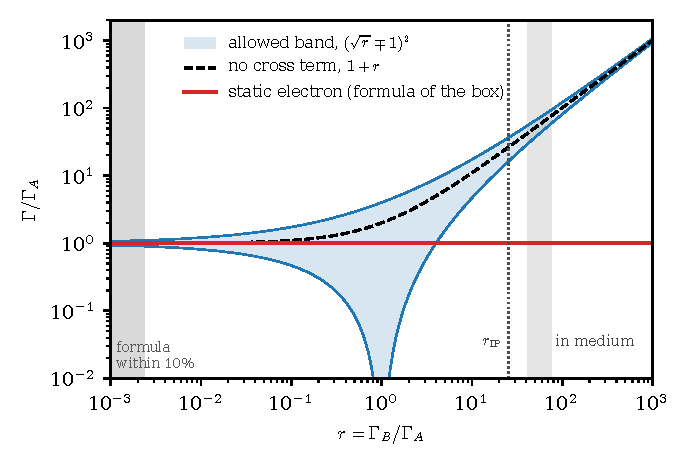
\includegraphics[width=0.82\linewidth]{figures/ch10/limit10_4a.pdf}
\captionof{figure}{Rate of $\mathcal{O}_8 = \vect{S}_\chi\cdot\vect{v}^\perp$ (spin-$\frac12$ dark matter, heavy mediator, elastic) relative to the static-electron formula of the box, $\varGamma_A$, against the ratio $r = \varGamma_B/\varGamma_A$ of the current-row rate $\varGamma_B$ to the formula. Blue: the band that positivity allows when the density--current cross term is not computed, $(\sqrt r \mp 1)^2$ (\cref{eq:10.4-band}). Dashed: $1 + r$, exact for responses averaged over the directions of $\vect{q}$, for which the cross term vanishes. Red: the formula. Gray at left: $r \le 2.4\times10^{-3}$, where every value in the band lies within \SI{10}{\percent} of the formula, $(\sqrt r + 1)^2 \le 1.1$. Dotted: silicon at $\mchi = \SI{10}{MeV}$ for independent particles, $r_{\mathrm{IP}} = 25.3$, from the empirical pseudopotential of Cohen and Bergstresser (model gap \SI{0.82}{eV}, $10^3$ $\vect{k}$ points, 36 conduction bands, bins of \SI{0.1}{eV}, 26-point average over directions, threshold \SI{1.11}{eV}, standard halo of \cref{sec:1.2}). Gray at right: the same ratio with the density row screened, $r_{\mathrm{IP}}\times2.31\times(1 \pm 0.3)$. The factor 2.31 is the screening of the density rate in the random-phase tables with local fields of \cref{sec:10.2}, and $\pm0.3$ the range allowed for the local-field change of the current row.}\label{fig:10-mixed-limit}
\par}
\smallskip
The formula leaves out the electron's own transverse motion, which in silicon carries about 25 times the rate the formula keeps, so the true rate is at least 16 times the formula for independent particles and at least 29 times with the density row screened.
\end{limitbox}

\subsection{Interference bound on a mixed block}\label{sec:10.4-band}

The rate of $\mathcal{O}_8$ shows how the rows combine. With the potentials of \cref{eq:8.1-O7O8} on the density and the current, the contraction \cref{eq:8.2-rate} has a density term, a current term and their interference. Continuity removes the parts along $\vect{q}$ on both sides (\cref{eq:D.30-O8T}). For elastic dark matter, and with the responses averaged over the directions of $\vect{q}$, the velocity integral is the one of \cref{app:A.8} with one change. The density term carries the dark matter's transverse velocity squared, $|\bar{\vect{v}}_{\mathrm{T}}|^2 = v^2 - \vmin^2$ on the energy shell, and its halo average is the second speed moment $\eta_2(\vmin) = 2\int_{\vmin}^\infty\dd v'\,v'\eta(v')$ in place of $\eta$ (\cref{eq:D.30-kernel}).
\begin{keyresult}[Rate of a velocity coupling]
For $\mathcal{O}_8$ with coefficient $c_8^{(e)}(q)$ and spin-$\frac12$ dark matter, the spectrum per unit target mass is
\begin{equation}
  \frac{\dd\mathcal{R}}{\dd\omega} = \frac{\rho_\chi}{16\pi^2\mchi\rho_T}\int\dd q\;q\,\bigl|c_8^{(e)}(q)\bigr|^2\Bigl[\underbrace{\eta_2(\vmin)\,\bar S_{nn}(q,\omega)}_{\text{electron at rest}} + \underbrace{\eta(\vmin)\,\Tr\bar S_{\vect{j}_{\mathrm{T}}\vect{j}_{\mathrm{T}}}(q,\omega)}_{\text{electron motion}}\Bigr] ,
  \label{eq:10.4-O8}
\end{equation}
with $\bar S$ averaged over the directions of $\vect{q}$, for which the density--current cross term vanishes. The first term is the rate of an electron at rest; the second is the electron's own transverse motion.
\end{keyresult}
\noindent The prefactor follows from \cref{eq:8.2-spectrum} with the kernel $\eta/(2q)$ per unit $\dd^3q/(2\pi)^3$ of \cref{eq:A.8-eta} and the factor $\frac14$ of the spin trace. For $c_8^{(e)} = \tilde V$ and $\Tr\bar S_{\vect{j}_{\mathrm{T}}\vect{j}_{\mathrm{T}}} = 0$, \cref{eq:10.4-O8} is the density rate with $\eta \to \eta_2/4$, the form of the box.

We can estimate the two terms before computing them. On the dark-matter side, the ratio $\eta_2/\eta$ is the mean of $|\bar{\vect{v}}_{\mathrm{T}}|^2$ over the particles fast enough to deposit $\omega$. It is $1.1\times10^{-6}$ at $\vmin = 0$, $1.0\times10^{-6}$ at $10^{-3}$ and $0.7\times10^{-6}$ at $2\times10^{-3}$, and it vanishes at the kinematic edge, where the only particles left move along $\vect{q}$. On the target side, the ratio $\Tr\bar S_{\vect{j}_{\mathrm{T}}\vect{j}_{\mathrm{T}}}/\bar S_{nn}$, integrated over $\omega$, is the mean transverse velocity squared of the electrons that make the pairs. In the empirical-pseudopotential model of silicon it is $3.2\times10^{-5}$ at $q_0$ and $2.1\times10^{-5}$ at $2q_0$, close to the free-gas value $\frac25v_{\mathrm{F}}^2 = 2.0\times10^{-5}$. At small $q$ it grows as $2\langle\omega^2\rangle/q^2$, the independent-particle form of \cref{eq:10.4-optical}: at $0.12\,q_0$ the model gives $4.1\times10^{-4}$ against $2\langle\omega^2\rangle/q^2 = 4.4\times10^{-4}$. We expect the electron term to exceed the dark-matter term by a factor of about 20 to 30, and more near the kinematic edge.

Let $\varGamma_A$ be the rate of the density term and $\varGamma_B$ the rate of the current term. The interference bound of \cref{sec:8.3} then limits the full rate whatever the cross term is.
\begin{keyresult}[Band on a mixed block]
For any target, halo and binning,
\begin{equation}
  \bigl(\sqrt{r} - 1\bigr)^2 \;\le\; \frac{\varGamma}{\varGamma_A} \;\le\; \bigl(\sqrt{r} + 1\bigr)^2 , \qquad r = \frac{\varGamma_B}{\varGamma_A} ,
  \label{eq:10.4-band}
\end{equation}
and with responses averaged over directions $\varGamma = \varGamma_A + \varGamma_B$. For independent particles $r$ is written $r_{\mathrm{IP}}$.
\end{keyresult}
\noindent The ratio of the two rates decides how much the cross term can matter. The half-width of the band relative to $1 + r$ is $2\sqrt r/(1 + r)$, below \SI{10}{\percent} only for $r < 2.5\times10^{-3}$ or $r > 4.0\times10^2$. For $r$ above 4 the lower edge exceeds one: the rate of an electron at rest is then an underestimate whatever the phase of the cross term. Positivity also says when the edges of the band are reached. Both edges need the density and current rows to be proportional on every final state the rate samples, and in an unpolarized crystal the two rows are far from proportional. In the model of silicon, along the generic direction $(5,3,1)$, the $\omega$-integrated cross block $|\vect{S}_{n\vect{j}_{\mathrm{T}}}|$ stays below 0.012 of $(S_{nn}\Tr S_{\vect{j}_{\mathrm{T}}\vect{j}_{\mathrm{T}}})^{1/2}$ up to $2.4\,q_0$, and on the two-, three- and fourfold axes it vanishes by symmetry. A crystal at fixed orientation keeps a cross term through the anisotropy of its response, the same anisotropy that makes the daily modulation of \cref{sec:11.7}.

In the medium the two terms of \cref{eq:10.4-O8} are screened differently. For a heavy mediator the density rate weighted with $\eta_2$ loses a factor 2.2 at \SI{30}{MeV}, 2.3 at \SI{10}{MeV} and 9.5 at \SI{1}{MeV} in the tables of \cref{sec:10.2}, while the current row changes only through local fields. Let screening lower the density rate by the factor $\varGamma_A/\varGamma_A^{\mathrm{med}}$ and change the current rate by the factor $1 + \delta^{j}_{\mathrm{LF}}$, the local-field correction of the transverse current averaged over the rate. Then
\begin{equation}
  r_{\mathrm{med}} = r_{\mathrm{IP}}\,\frac{\varGamma_A}{\varGamma_A^{\mathrm{med}}}\,\bigl(1 + \delta^{j}_{\mathrm{LF}}\bigr) ,
  \label{eq:D.30-rmed}
\end{equation}
and $r_{\mathrm{med}} \ge r_{\mathrm{IP}}$ whenever the product of the two factors is at least one. Since the lower edge of \cref{eq:10.4-band} increases with $r$ for $r \ge 1$, $(\sqrt{r_{\mathrm{med}}} - 1)^2 \ge (\sqrt{r_{\mathrm{IP}}} - 1)^2$ under the same condition.

\begin{workedexample}{The band for a velocity coupling in silicon}\label{we:10-band}
Take $\mathcal{O}_8$ with a heavy mediator, $\mchi = \SI{10}{MeV}$, the halo of \cref{sec:1.2} and the threshold $\Eg = \SI{1.11}{eV}$ of the tables of \cref{sec:10.2}. Averaged over directions with a 26-point rule, the empirical-pseudopotential model provides the two integrals of \cref{eq:10.4-O8} for independent particles. Their ratio is
\begin{equation*}
  r_{\mathrm{IP}} = \frac{\int\dd\omega\int\dd q\,q\,\eta\,\Tr\bar S^0_{\vect{j}_{\mathrm{T}}\vect{j}_{\mathrm{T}}}}{\int\dd\omega\int\dd q\,q\,\eta_2\,\bar S^0_{nn}} = 25.3 .
\end{equation*}
The model's gap is \SI{0.82}{eV}; shifting all its pair energies up so that the model gap becomes \SI{1.11}{eV} changes $r_{\mathrm{IP}}$ by \SI{2}{\percent}. With $\sqrt{r_{\mathrm{IP}}} = 5.03$, \cref{eq:10.4-band} puts the rate between $(5.03 - 1)^2 = 16.2$ and $(5.03 + 1)^2 = 36.4$ times the rate of an electron at rest, and the direction-averaged value is $1 + r_{\mathrm{IP}} = 26.3$. The rate of the density row alone is low by more than an order of magnitude.

Now screen. With the random-phase tables with local fields of \cref{sec:10.2}, the density rate weighted with $\eta_2$ falls by a factor 2.31 at this mass, the same as with $\eta$ (2.30). The local-field change of the current row is not known for silicon; the model finds $-4$ to $-15$ percent at $q_0$ and $2q_0$, and we allow $\pm30$ percent. Then $r_{\mathrm{med}} = 25.3\times2.31\times(1 \pm 0.3)$ lies between 41 and 76, the lower edge of the band between 29 and 60, and the direction-averaged rate is 42 to 77 times the static-electron formula with the same screened density row. The two models in this estimate differ: the current comes from the empirical pseudopotential, the screening of the density from a Kohn--Sham calculation. At $q_0$ and \SI{5}{eV} the model itself lowers $S_{nn}$ to 0.22 of its unscreened value, in line with the tables.

The ratio grows toward small masses, since the dark matter's transverse velocity vanishes at the kinematic edge: $r_{\mathrm{IP}} = 22$ at \SI{30}{MeV}, 33 at \SI{5}{MeV}, 56 at \SI{3}{MeV} and about 150 at \SI{2}{MeV}. The model's plane waves end at $2.8\,q_0$, while \SI{29}{\percent} of the screened heavy-mediator rate of silicon at \SI{10}{MeV} comes from $q > 2q_0$ (\cref{sec:10.2-corrections}). At large $q$ the ratio of the two responses tends to the mean transverse velocity squared of the valence electrons, which the model puts at $2\times10^{-5}$ to $3\times10^{-5}$ and which the core-region oscillations missing from pseudo-wavefunctions can only raise. The value of $r_{\mathrm{IP}}$ above is, if anything, low.
\end{workedexample}

The local-field screening of the transverse current in silicon is not known. Estimates put it at 10 to \SI{30}{\percent} (\cref{app:E.16}), the model above at 4 to \SI{15}{\percent}, both of the sign that lowers the current. The unknown local-field screening leaves open the factor between the static-electron formula and the true rate of $\mathcal{O}_8$, $\mathcal{O}_5$ or $\mathcal{O}_2$, or of the spin operators that carry $\vect{v}^\perp$. \Cref{eq:10.4-band} bounds the factor from below but does not fix it. Until the local-field screening of the transverse current is computed, limits set on these operators with the density response alone are conservative by at least an order of magnitude; these operators need a material input beyond the density response.
